\documentclass[10pt]{article}
\usepackage{textcomp, graphicx,amssymb, amstext, amsmath, epstopdf, booktabs, verbatim, geometry, appendix, natbib, lmodern, float, tabularx, color}

\geometry{letterpaper}
\usepackage{etoolbox}


\usepackage[utf8]{inputenc}
\usepackage{listings}

\definecolor{codegreen}{rgb}{0,0.6,0}
\definecolor{codegray}{rgb}{0.5,0.5,0.5}
\definecolor{codepurple}{rgb}{0.58,0,0.82}
\definecolor{backcolour}{rgb}{0.95,0.95,0.92}

\lstdefinestyle{mystyle}{
    backgroundcolor=\color{backcolour},
    commentstyle=\color{codegreen},
    keywordstyle=\color{magenta},
    numberstyle=\tiny\color{codegray},
    stringstyle=\color{codepurple},
    basicstyle=\footnotesize,
    breakatwhitespace=false,
    breaklines=true,
    captionpos=b,
    keepspaces=true,
    numbers=left,
    numbersep=5pt,
    showspaces=false,
    stringstyle=\color{codepurple},
    showstringspaces=false,
    showtabs=false,
    tabsize=2
}

\lstset{style=mystyle}

\usepackage{hyperref}
\usepackage{tikz}
\usetikzlibrary{positioning, arrows.meta, calc, fit}

%-----------------------------------------------------------
\newcommand*{\Title}{AgentDesign: Hermes Profile Architecture}
\newcommand*{\cpiType}{Math \& Librarian Profiles --- Design Documentation}
\newcommand*{\Date}{September 2026}
\newcommand*{\Author}{Mehdi Ghasemi}
\newcommand*{\Company}{Research Workspace}
\newcommand*{\Us}{M. Ghasemi}

\newbool{Toptal}
\setbool{Toptal}{false}
\newbool{Guidelines}
\setbool{Guidelines}{false}
\newbool{Proposal}
\setbool{Proposal}{true}

\definecolor{DarkBlue}{rgb}{0,0.2,0.6}
\definecolor{PinkPurple}{rgb}{0.8,0.3,0.3}
\ifbool{Toptal}{
	\hypersetup{
		pdftitle={Project Proposal},
		colorlinks=true,
		linkcolor=toptalGreen,
		filecolor=toptalGreen,
		urlcolor=toptalGreen,
		pdfauthor={Mehdi Ghasemi}
	}
}{
	\hypersetup{
		pdftitle={AgentDesign: Hermes Profile Architecture},
		colorlinks=true,
		linkcolor=DarkBlue,
		filecolor=PinkPurple,
		urlcolor=PinkPurple,
		pdfauthor={Mehdi Ghasemi}
	}
}

\title{\Title}
\author{\Author}
\date{\Date}
%-----------------------------------------------------------
\usepackage{gensymb}
\usepackage{textcomp} % \textless/\textgreater: bare < > are T1 accents under the cpi template and break compilation
\usepackage{pifont} % \ding for enabled/disabled marks (\mkE, \mkD)
\usepackage{cpistuff/cpi} % This is what makes your document look like a cpi document.

% small helpers for this document — MUST come after cpistuff/cpi (it redefines \mono)
\newcommand{\mono}[1]{{\ttfamily\small #1}}
\definecolor{mathgreen}{RGB}{26,93,58}
\definecolor{libbrown}{RGB}{93,58,30}
\newcommand{\mkE}{\textcolor{mathgreen}{\ding{51}}}       % enabled
\newcommand{\mkD}{\textcolor{PinkPurple}{\ding{55}}}      % disabled
\newcommand{\mkA}{$-$}                                    % absent

\begin{document}

\begin{titlepage}
\maketitle
\end{titlepage}

\linespread{1.2}

\begin{executive}

This document records the complete design of the two Hermes agent profiles that power my
mathematical research workflow --- \textbf{\mono{math}} and \textbf{\mono{librarian}} --- and
specifies an abstraction layer under which either profile can be re-pointed at any future math
project without modification. All facts are extracted from the live configuration on
\texttt{/home/mehdi/.hermes/profiles/} (config version 49, September 2026); every claim in
Sections~\ref{sec:profiles}--\ref{sec:defects} is verifiable against the files listed in
Section~\ref{sec:sources}.

The architecture resolves into five layers: a shared \emph{Hermes core}, an isolated
\emph{profile system}, a \emph{skill catalog} (57--59 skills, capability-gated per profile),
an \emph{MCP bridge} (13 registered servers, one generic CLI-adapter pattern covering 8 of them),
and an \emph{external service plane} on the local network. The math profile is a full-stack
researcher with a 5.9\,GB sandboxed toolchain environment; the librarian profile is a
capability-degraded derivative that shares every registration but disables all computational
skills and adds two ingestion skills of its own.

Two structural findings drive the abstraction design: (i)~the librarian profile's MCP servers
import scripts from the math profile's directory tree, so it cannot exist without the math
profile; and (ii)~both profiles contain a stale reference to \mono{IreneRewrite}, deleted when
that worktree was merged into \mono{Irene} on 2026-09-18. Section~\ref{sec:abstraction}
proposes a capability/manifest model --- persona templates, path interpolation, a shared adapter,
a service registry, and per-project binding files --- that removes every identified coupling in
five concrete steps.

\end{executive}

\tableofcontents
\newpage

%=====================================================================
\section{Objectives and Scope}\label{objectives}

The \mono{AgentDesign} project has three objectives:

\begin{enumerate}
    \item \textbf{Document the as-is architecture.} Record, with file-level evidence, how the
    math and librarian profiles are composed: directory layout, configuration sections, skill
    catalogs, MCP server registrations, external services, scheduled jobs, and state stores.
    This is Sections~\ref{sec:layers}--\ref{sec:workflow}.
    \item \textbf{Identify the coupling points.} Enumerate every place where a profile depends
    on the specific current project layout --- absolute paths, cross-profile imports, hardcoded
    endpoints, and stale references --- so that the design of record distinguishes what is
    load-bearing from what is incidental (Section~\ref{sec:defects}).
    \item \textbf{Specify an abstraction layer.} Define how profiles become reusable personas:
    independent of any particular math project, instantiable for a new project with zero or one
    line of configuration, and testable against a capability contract
    (Section~\ref{sec:abstraction}).
\end{enumerate}

The scope is the two active research profiles. The remaining four registered profiles
(\mono{default}, \mono{coder}, \mono{advisor}, \mono{trader}) are out of scope; their existence
is noted only in Section~\ref{sec:profiles}. This project does not modify any live profile
configuration --- it is a documentation and design artifact.

%=====================================================================
\section{Layered Architecture}\label{sec:layers}

Figure~\ref{fig:layers} gives the visual layout of the infrastructure under which both profiles
operate. Five layers are distinguished; each lower layer is shared, each upper layer is isolated
per profile at \mono{\textasciitilde/.hermes/profiles/\textless name\textgreater/}.

\begin{figure}[H]
\centering
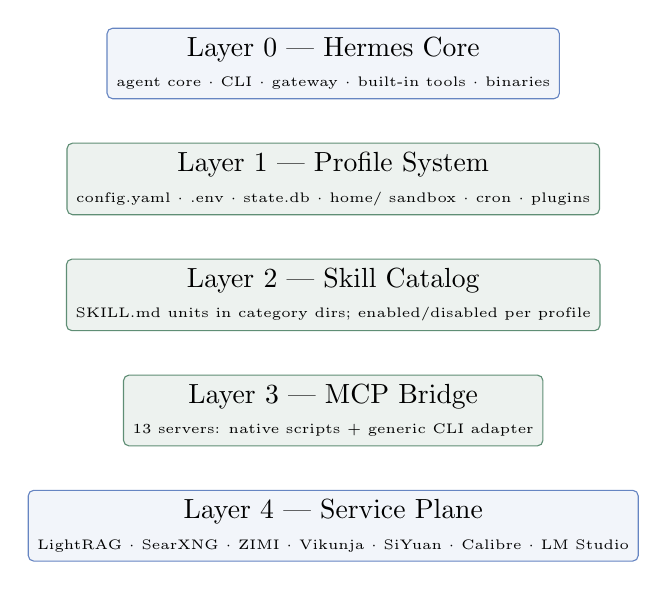
\begin{tikzpicture}[
    boxL/.style={draw=DarkBlue!60, fill=DarkBlue!5, rounded corners=2pt, minimum width=3.1cm, align=center},
    boxP/.style={draw=mathgreen!70, fill=mathgreen!8, rounded corners=2pt, minimum width=3.1cm, align=center},
    layerLbl/.style={font=\small\bfseries, text=DarkBlue},
    every edge/.style={->, >=Stealth, draw=codegray}
  ]
  \node[boxL] (core) {Layer 0 --- Hermes Core\\[-1pt]\tiny agent core $\cdot$ CLI $\cdot$ gateway $\cdot$ built-in tools $\cdot$ binaries};
  \node[boxP, below=.55cm of core] (prof) {Layer 1 --- Profile System\\[-1pt]\tiny config.yaml $\cdot$ .env $\cdot$ state.db $\cdot$ home/ sandbox $\cdot$ cron $\cdot$ plugins};
  \node[boxP, below=.55cm of prof] (skill) {Layer 2 --- Skill Catalog\\[-1pt]\tiny SKILL.md units in category dirs; enabled/disabled per profile};
  \node[boxP, below=.55cm of skill] (mcp) {Layer 3 --- MCP Bridge\\[-1pt]\tiny 13 servers: native scripts + generic CLI adapter};
  \node[boxL, below=.55cm of mcp] (svc) {Layer 4 --- Service Plane\\[-1pt]\tiny LightRAG $\cdot$ SearXNG $\cdot$ ZIMI $\cdot$ Vikunja $\cdot$ SiYuan $\cdot$ Calibre $\cdot$ LM Studio};
\end{tikzpicture}
\caption{Five-layer profile architecture. Layers 2--3 are the capability surface of a profile;
layers 0 and 4 are shared infrastructure. Arrows indicate the direction in which each layer is
configured by, or depends on, the layer above it.}\label{fig:layers}
\end{figure}

\subsection*{Layer 0 --- Hermes Core}
The core lives at \mono{\textasciitilde/.hermes/hermes-agent/}: agent runtime, CLI (profile
switching, tool registry), platform gateway (Telegram/WhatsApp/webhook adapters), built-in tools
(terminal, browser, vision, file I/O, web search, kanban, memory) and the MCP discovery layer
(\mono{tools/mcp\_tool\_*.py}). Shared binaries (\mono{tirith} security scanner, \mono{uv}, Python
3.14, Node 26, ripgrep, Chromium) live in \mono{\textasciitilde/.hermes/tools/}; all MCP stdio
servers run from a single shared virtualenv at \mono{\textasciitilde/.hermes/mcp-servers/.venv/}.

\subsection*{Layer 1 --- Profile System}
Each profile is an isolated directory with its own configuration, credentials, state and sandbox.
The two profiles under study:

\begin{itemize}
    \item \textbf{\mono{math}} (8.4\,GB; 493 sessions): full-stack mathematical researcher.
    Working directory \mono{/home/mehdi/Code/Python/}. Carries a 5.9\,GB sandboxed home
    environment with the complete local toolchain (Section~\ref{sec:profiles}). Active Telegram
    gateway; five cron jobs registered (two enabled). Kanban orchestrator and default assignee is \mono{math}.
    \item \textbf{\mono{librarian}} (174\,MB; 8 sessions): literature manager --- ``manage and
    maintain books and articles.'' Working directory \mono{/home/mehdi/Code/}. Empty \mono{home/}
    stub, no cron jobs, no gateway platforms. Shares the same kanban assignment (\mono{math}), which
    is itself a coupling noted in Section~\ref{sec:defects}. It is also the only profile with an active
    metrics sender: its \mono{telemetry.shared\_metrics} block has both \mono{enabled} and \mono{send}
    set to true; math's config carries no telemetry block at all.
\end{itemize}

Both profiles run the same local model: \mono{qwen3.8-27b} via LM Studio at
\mono{http://localhost:1234/v1}, with an \mono{on\_session\_start} hook
(\mono{\textasciitilde/.hermes/agent-hooks/ensure-lmstudio.sh}) that guarantees the model server
is up before each session. Long-term memory in both profiles is backed by Honcho
(\mono{memory.provider: honcho}, service at port 8008).

\subsection*{Layer 2 --- Skill Catalog}
Skills are Markdown-defined capability units (\mono{SKILL.md} with YAML frontmatter), organized
in category directories, optionally carrying scripts and credential files. Each profile holds 57
skill units across nine named categories plus a handful of top-level skills (union: 59); the full
per-profile inventory is in \mono{references/skill\_inventory.md}; Section~\ref{sec:skills} summarizes
the design-relevant parts.

\subsection*{Layer 3 --- MCP Bridge}
Skills reach services either directly (terminal/shell) or through Model Context Protocol servers
registered under \mono{mcp\_servers:} in each profile's config; every registered tool is exposed
to the model as \mono{mcp\_\_\textless server\textgreater\_\_\textless tool\textgreater} (e.g.\ \mono{mcp\_\_vikunja\_\_tasks\_\_create}). Section~\ref{sec:mcp} documents the two server
families and the cross-profile dependency this layer creates.

\subsection*{Layer 4 --- Service Plane}
A fixed set of self-hosted services on the local network (host \mono{192.168.1.70}, DDNS fallback
\mono{mghasemi.ddns.net}), plus two SaaS APIs and one local inference server. Table~\ref{tab:services}
lists them with their role in the workflow.

%=====================================================================
\section{Profile System: Structure Comparison}\label{sec:profiles}

Table~\ref{tab:profilecmp} compares the structural elements of the two profiles. All values were
read directly from \mono{\textasciitilde/.hermes/profiles/\textless p\textgreater/} in September 2026.

\begin{table}[H]
\centering\small
\caption{Structural comparison, math vs.\ librarian profile.}\label{tab:profilecmp}
\renewcommand{\arraystretch}{1.15}
\begin{tabularx}{\textwidth}{@{}l X X@{}}
\toprule
Element & \textbf{\mono{math}} & \textbf{\mono{librarian}}\\
\midrule
config version & 49 & 49\\
Model / provider & qwen3.8-27b / lmstudio & qwen3.8-27b / lmstudio (+explicit \mono{chat\_completions} api mode)\\
Terminal cwd & \mono{/home/mehdi/Code/Python/} & \mono{/home/mehdi/Code/}\\
\mono{.env} size & 52 lines, 49 keys & 45 lines, 42 keys (strict subset of math; no Telegram/WhatsApp/OpenRouter)\\
Skills (\mono{SKILL.md}) & 57 across 9 named categories + top-level (9 further empty category shells) & same shape; 2 skills unique to each (librarian: \mono{calibre-library-ingestion}, \mono{djvu-to-pdf}; math: \mono{exact-symbolic-gate-scripts}, \mono{irene-rewrite-dev})\\
\mono{skills.disabled} entries & 12 & 28 (superset: all computational + dev skills)\\
MCP servers registered & 13 & 13 (identical names; two differ in content, Table~\ref{tab:mcp})\\
Sandbox \mono{home/} & 5.9\,GB toolchain env (Table~\ref{tab:homeenv}) & empty directory\\
\mono{bin/} & tirith, uv, uvx & tirith only\\
\mono{scripts/} & \mono{mcp\_cli\_adapter.py} + wiki pipeline (8 further \mono{.py}) & \textbf{absent}\\
\mono{plugins/} dir & hermes-android, vikunja, wiki-browser & empty\\
Enabled plugins (config) & vikunja, wiki-browser & vikunja, wiki-browser (installed under shared \mono{\textasciitilde/.hermes/plugins/})\\
Cron jobs & 5 registered (2 enabled: arXiv scan every 10\,080\,min; Wiki Maintenance weekly Sundays 03:00 --- named ``bi-weekly'' but the cron is \texttt{0 3 * * 0}) & none (no \mono{jobs.json}; ticker state only)\\
Sessions in state.db & 493 & 8\\
Kanban orchestrator / assignee & \mono{math} / \mono{math} & \mono{math} / \mono{math}\\
Code execution mode & \mono{project} & \mono{project}\\
Approvals mode & off (600\,s timeout) & off\\
Compression threshold & --- & 0.6\\
Telemetry block & absent & present (\mono{shared\_metrics}, \textbf{send=true} --- the only profile transmitting metrics)\\
Desktop repo scan roots & \mono{/home/mehdi/Code/Python/} & \mono{/home/mehdi/Code/}\\
Total profile size & 8.4\,GB & 174\,MB\\
\bottomrule
\end{tabularx}
\end{table}

\textbf{The librarian is a capability-degraded derivative of math}, not an independent design: it
inherits every skill directory and MCP registration, then suppresses the computational surface via
the \mono{skills.disabled} list. It also carries two skills that exist only in its own tree ---
\mono{calibre-library-ingestion} and \mono{djvu-to-pdf} (productivity category) --- which is where
its genuine specialization lives.

The math sandbox home environment, the single largest structural asymmetry:

\begin{table}[H]
\centering\small
\caption{Contents of \mono{\textasciitilde/.hermes/profiles/math/home/} (5.9\,GB). The profile home is a
partial toolchain plus package caches: Lean 4 lives here; SageMath and TeXLive resolve to host-level
installs (\texttt{/usr/bin/pdflatex}, \mono{miniconda3/envs/sage}).}\label{tab:homeenv}
\renewcommand{\arraystretch}{1.12}
\begin{tabularx}{\textwidth}{@{}l X@{}}
\toprule
Directory & Role\\
\midrule
\mono{.elan/} (2.9\,GB) & Lean 4 toolchain \mono{leanprover--lean4---v4.31.0} used by the lean4 MCP server\\
\mono{.rustup/} (1.4\,GB), \mono{.cargo/} & Rust stable-x86\_64 toolchain plus registry and download caches\\
\mono{.cache/} (1.2\,GB) & Package/browser caches: ms-playwright (674\,MB), pip (517\,MB) --- not a toolchain\\
\mono{.npm/} (355\,MB) & npm cache for the sandboxed node 26 environment\\
\mono{.notebooklm/} (21\,MB) & Dedicated Chrome profile for NotebookLM grounded synthesis\\
\mono{.texlive2023/} (14\,MB) & texmf-var font/format caches only; actual TeXLive is host-level\\
\mono{.sage/}, \mono{.maxima/} & SageMath runtime state directories (binary resolves to host conda env)\\
\mono{wiki/} (28\,KB) & Small local wiki with SCHEMA.md index --- distinct from the main 149\,MB wiki at \mono{/home/mehdi/Code/wiki}\\
\mono{.ssh/}, \mono{.gitconfig}, \mono{.bashrc} & Identity and shell configuration of the sandboxed user\\
\mono{pb\*.py}, \mono{wiki\_ingest\*.py}, \mono{pb\_token.txt} & PocketBase + wiki ingestion pipeline scripts (9 files)\\
\bottomrule
\end{tabularx}
\end{table}

\noindent Two facts matter for the abstraction design. First, the 5.9\,GB figure is inflated by roughly
1.7\,GB of disposable package caches (\mono{.cache/}, \mono{.npm/}); the load-bearing toolchain state is
Lean under \mono{.elan/} and Rust under \mono{.rustup/}. Second, SageMath and TeXLive were never actually
installed in this home --- the sagemath MCP server falls through its candidate list to a host conda env,
and \texttt{pdflatex} comes from \texttt{/usr/bin} --- so the profile home is not a self-contained
computation environment despite looking like one.

%=====================================================================
\section{Skill System: Design for General Math Projects}\label{sec:skills}

Skills are the unit of reusability. Each \mono{SKILL.md} carries a trigger description in its
frontmatter, an imperative body, optional scripts, and --- where needed --- a co-located
credential file (\mono{.emv}; two exist under math --- \mono{skills/productivity/siyuan/.emv}
and \mono{plugins/vikunja/dashboard/.emv} --- and one under librarian). The catalog is shared
between the two profiles (same 24 top-level skill directories: nine sub-skill categories, six
top-level skills in math / five in librarian, and nine empty category shells); only activation
differs. Table~\ref{tab:skillcats} summarizes by category; \textbf{E}/\textbf{D}/$-$ = enabled / disabled / absent per profile
(counts from \mono{references/skill\_inventory.md}).

\begin{table}[H]
\centering\small
\caption{Skill catalog by category (E/D counts of skills present in the profile tree).}\label{tab:skillcats}
\renewcommand{\arraystretch}{1.12}
\begin{tabularx}{\textwidth}{@{}l l X@{}}
\toprule
Category & Counts (math / lib) & Design role\\
\midrule
research & 24E/1D $\;\vert$\; 18E/6D & Core literature + computation surface: \mono{math-research-workflow} (the 6-stage pipeline), \mono{sagemath-mcp}, \mono{sympy-mcp}, \mono{lean4}, \mono{lean4-goedel-agent}, \mono{lightrag}, \mono{searxng}, \mono{zimi}, \mono{wolfram-alpha}, \mono{academic-research-hub}, \mono{arxiv}, wiki pipeline skills; math-only: \mono{exact-symbolic-gate-scripts}\\
productivity & 7E/1D $\;\vert$\; 7E/3D (8 / 10 total) & Knowledge management: \mono{vikunja}, \mono{siyuan}, \mono{zotero}, \mono{calibre} (disabled in both), \mono{latex-manuscript}, \mono{project-bib}, \mono{ocr-and-documents}; librarian adds \mono{calibre-library-ingestion}, \mono{djvu-to-pdf}\\
mlops & 3E/1D $\;\vert$\; 2E/2D & Local inference ops: \mono{lmstudio-configuration}, \mono{pocketbase}, \mono{dsdp-extension-workflow} (librarian disabled)\\
software-development & 6E $\;\vert$\; 4E/2D & Hermes self-extensibility, planning, subagent orchestration, desktop DOM inspection\\
github / devops / autonomous-ai-agents / web & e.g.\ github 1E/1D $\vert$ 0E/2D & Repo ops, SDLC review (lib disabled), merge-reconciler, blocked-page recovery\\
social-media & 0E/1D $\;\vert$\; 1E/0D & \mono{reddit-reading} --- inverted gate: off for math, on for librarian\\
top-level skills & 6E $\;\vert$\; 3E/2D & \mono{differential-sdp}, \mono{ghasemi-latex-style}, \mono{hermes-plugin-management}, \mono{semantic-scholar}, \mono{workspace-doc-hierarchy}; math adds \mono{irene-rewrite-dev} (librarian disables it)\\
\bottomrule
\end{tabularx}
\end{table}

Three observations are design-relevant:

\begin{enumerate}
    \item \textbf{The math research surface is exactly the set of skills a generic math project
    needs}: decompose $\to$ literature $\to$ compute $\to$ verify $\to$ write, implemented by
    \mono{math-research-workflow}, which names 18 sibling skills in its frontmatter --- 17 of them
    live catalog entries, the eighteenth (\mono{simplerag-memory}) dead. This set, not the full
    catalog, defines the reusable ``mathematician'' capability contract
    (Section~\ref{sec:abstraction}).
    \item \textbf{The librarian's disabled list is a negative specification of that same
    contract}: every computational skill (\mono{sagemath-mcp}, \mono{sympy-mcp},
    \mono{lean4}, \mono{lean4-goedel-agent}, \mono{scientific-coding}), the DSDP skills, and the
    Irene/dev skills are turned off. Capability gating by negation works today but is brittle in a
    subtler way than it looks: entries resolve by \emph{leaf name} against the profile's skill tree,
    which includes the curator tombstone directory \mono{skills/.archive/}. All 40 disabled names
    (12 math + 28 librarian) therefore resolve to a real \mono{SKILL.md}; none dangles. But 6 of
    math's and 9 of the librarian's entries resolve \emph{only} under \mono{.archive/} --- they are
    residue from skills the curator has already retired (e.g.\ \mono{docx}, \mono{opencode},
    \mono{test-driven-development}; for the librarian also \mono{irene-rewrite-dev}, which exists as
    an \emph{active} top-level skill in math while pointing at a librarian tombstone). Because
    resolution is name-based, any of these 15 stale entries would silently disable a same-named
    skill if it were ever reinstalled. One inversion deserves note: \mono{reddit-reading} is
    disabled for math but enabled for librarian --- the only skill whose gate runs opposite to every
    other difference between the two profiles.
    \item \textbf{One reference is stale}: \mono{math-research-workflow} names
    \mono{simplerag-memory} ten times (frontmatter plus nine body references), eight of them shell
    invocations of a nonexistent \mono{simplerag\_client.sh}; no such skill exists in either
    profile tree or in the bundled pool.
\end{enumerate}

%=====================================================================
\section{MCP Bridge}\label{sec:mcp}

Thirteen MCP servers are registered per profile, all launched with the shared interpreter
\mono{\textasciitilde/.hermes/mcp-servers/.venv/bin/python}. They fall into three families:

\begin{table}[H]
\centering\small
\caption{MCP server registrations. ``Pattern'' distinguishes native servers from generic CLI-adapter
wraps; the script path is as written in each profile's config (identical strings for both profiles
except where noted).}\label{tab:mcp}
\renewcommand{\arraystretch}{1.12}
\begin{tabularx}{\textwidth}{@{}l l X c@{}}
\toprule
Server & Pattern & Script (path relative to) & Tools\\
\midrule
sagemath & native & \mono{profiles/math/skills/research/sagemath-mcp/} & 10\\
lean4 & native & \mono{profiles/math/skills/research/lean4/} & 4\\
searxng & native & \mono{profiles/math/skills/research/searxng/scripts/} & 1\\
vikunja & CLI adapter & tool: \mono{profiles/math/skills/productivity/vikunja/} & 15\\
wolfram-alpha & CLI adapter & \mono{.../research/wolfram-alpha/} & 3\\
lightrag-query & CLI adapter & \mono{.../research/lightrag/} & 3\\
siyuan & CLI adapter & \mono{.../productivity/siyuan/} & 7\\
zimi & CLI adapter & \mono{.../research/zimi/} & 4\\
zotero & CLI adapter & \mono{.../productivity/zotero/} & 7\\
scientific-coding & CLI adapter & \mono{.../research/scientific-coding/} (CPU/mem sandbox limits via env) & 4\\
latex-manuscript & CLI adapter & \mono{.../productivity/latex-manuscript/} (compile, AST check, glossary, notation audit, diff-patch) & 5\\
hermes-irene & direct script & \mono{Code/Python/IreneRewrite/scripts/hermes\_mcp\_tool.py} --- \textbf{path no longer exists} (worktree merged into \mono{Irene}, folder deleted 2026-09-18; file never committed to git) & $-$ \\
calibre & native (librarian only, active) & math: env block only, no command; librarian: \mono{Code/Python/tools/calibre-mcp/server.py} with its own venv, base URL \mono{:9876}, timeout 300\,s & 12\\
\bottomrule
\end{tabularx}
\end{table}

The \textbf{generic CLI-adapter pattern} is the load-bearing design of this layer. One script ---
\mono{profiles/math/scripts/mcp\_cli\_adapter.py} --- wraps any argparse-based Python CLI tool as a
stdio MCP server: it introspects the target's parser at startup, exposes each subcommand as an MCP
tool with JSON-schema arguments, and reconstructs command lines from tool calls. Eight of thirteen
servers use it; adding a new service-backed skill therefore requires only a thin CLI script plus a
config entry (URL/token via env), no protocol code.

Two cross-profile facts follow directly from the table:

\begin{itemize}
    \item Every path in every MCP registration --- including all of the librarian's --- points into
    the \textbf{math profile's directory tree}: 8 \mono{TOOL\_SCRIPT} values, 3 native server
    scripts, and the adapter itself (\mono{profiles/math/scripts/mcp\_cli\_adapter.py}). The
    librarian has no \mono{scripts/} directory of its own. Deleting or moving the math profile would
    silently break every tool-bridged capability of the librarian.
    \item Both profiles register \mono{hermes-irene} against a script inside
    \mono{IreneRewrite}, which was merged into \mono{Irene} and deleted on 2026-09-18; in math it is
    \mono{enabled: false} (dormant), in librarian \mono{true} (broken at startup). The correct target
    after the merge would live under \mono{/home/mehdi/Code/Python/Irene/}, where no such script has
    yet been created.
\end{itemize}

%=====================================================================
\section{Tool Stack and Service Plane}\label{sec:services}

Table~\ref{tab:services} lists the services both profiles reach, grouped by role in the research
workflow. All self-hosted endpoints share host \mono{192.168.1.70} (fallback
\mono{mghasemi.ddns.net}); credentials live in each profile's \mono{.env} (42 shared keys; 7
math-only, all messaging/auxiliary: Telegram bot token and allowlist, WhatsApp mode fields,
OpenRouter key).

\begin{table}[H]
\centering\small
\caption{Service plane. Both profiles share the same registrations; differences noted.}\label{tab:services}
\renewcommand{\arraystretch}{1.12}
\begin{tabularx}{\textwidth}{@{}l l X c@{}}
\toprule
Service & Endpoint & Role in workflow & MCP\\
\midrule
LightRAG & :9621 (API key) & Graph-RAG over the curated literature lake: ingest + multi-hop query & yes $\times$1 profile \\
SearXNG & :5050 & Federated web metasearch, structured JSON output & yes\\
ZIMI & :8899 & Offline encyclopedia (Wikipedia ZIM) for archival grounding before live search & yes\\
Vikunja & :3456 (token) & Task ledger: hypothesis trees, phase tracking, cross-session state & yes + plugin\\
SiYuan & :6806 (token) & Block-level notes; human-readable findings and equation blocks; .emv credential co-located in skill dir & yes + plugin\\
Calibre-web / Calibre MCP & :9876 & Ebook library management --- active for librarian only (12 tools); math has env block without command & lib. only\\
Zotero & API (key) & Bibliography, BibTeX export, citation verification & yes\\
Wolfram\textbar Alpha & SaaS API (appid) & Symbolic/numeric computation beyond local Sage/SymPy & yes\\
Honcho & :8008 & Persistent cross-session research memory (both profiles' \mono{memory.provider}) & built-in tools\\
LM Studio & localhost:1234 (\mono{.env} points at 192.168.1.81:1234) & Local inference for both profiles; ensured by session-start hook & --- (model provider)\\
Portainer & :9000 (API key) & Container management of the service plane itself & via terminal\\
Semantic Scholar / arXiv Crossref & SaaS APIs & Citation-graph layer and metadata verification gate (skills, not MCP servers) & via skills\\
\bottomrule
\end{tabularx}
\end{table}

The \textbf{four integration channels} a skill may use, in the preference order codified by
\mono{math-research-workflow}:

\begin{enumerate}
    \item \emph{MCP native / adapter tools} --- fastest path into services; no shell involved.
    \item \emph{Terminal invocations of CLI scripts} bundled with skills (e.g.\ the arXiv research
    script, wiki ingestion pipeline).
    \item \emph{Built-in Hermes tools} --- web search/extraction, file I/O, browser automation.
    \item \emph{Local binaries from the sandbox home} (SageMath, Lean 4 via elan/rustup, TeXLive)
    for computation and compilation that must stay on-machine.
\end{enumerate}

%=====================================================================
\section{The Research Workflow}\label{sec:workflow}

The designated workflow for math projects is the \textbf{\mono{math-research-workflow}} skill
(v1.6), a single-agent adaptation of the MathAgent multi-agent system with Graph-of-Agents message
passing and Reflexion quality gates. Its six stages, each gated by a 5-check Reflexion gate:

\begin{center}
\small
\renewcommand{\arraystretch}{1.2}
\begin{tabularx}{\textwidth}{@{}c X l@{}}
\toprule
Stage & Activity & Primary tools\\
\midrule
1. Problem decomposition & Restate the problem; open Vikunja tasks and a hypothesis tree (conjecture = parent, attack branches = children with status) & vikunja MCP\\
2. Literature synthesis & Local-first retrieval cascade: LightRAG $\to$ academic-research-hub $\to$ Semantic Scholar $\to$ SearXNG $\to$ ZIMI; every citation passes the \emph{Citation Verification Gate} (arXiv API / Crossref / S2 before any bibliographic fact is recorded) & lightrag, searxng, zimi, s2 skill\\
3. Computation & Deterministic-first: SymPy $\to$ SageMath $\to$ Wolfram\textbar Alpha $\to$ sandboxed scientific-coding; Error-Feedback Loop with a 3-retry budget, exact prior error carried into each retry & sympy-mcp, sagemath-mcp, wolfram-alpha, scientific-coding\\
4. Formal verification & Three-stage Lean pipeline: formalize $\to$ compile clean (\mono{lean4\_check} against an explicit Mathlib project) $\to$ statement-fidelity diff vs.\ the informal claim; only then is a theorem ledger-marked ``proven \& Lean-verified'' & lean4, lean4-goedel-agent\\
5. Manuscript production & Drafter $\to$ Enhancer $\to$ Reviewer pass over LaTeX with the ghasemi-latex-style anti-pattern checklist and notation audit & latex-manuscript MCP, ghasemi-latex-style\\
6. Reflection \& close-out & Claims ledger updated; failures promoted to skill pitfalls or project reports; project README + AGENTS.md status synced in the same commit & ---\\
\bottomrule
\end{tabularx}
\end{center}

Supporting state: a per-project failure scratchpad at
\mono{\textasciitilde/.hermes/profiles/math/scratchpad/\textless problem\textgreater/failures.md},
per-project verified-source registries for citation dedup, and the cron jobs (weekly arXiv scan in
the five-topic overlap set; bi-weekly wiki maintenance) that feed Stage~2 continuously. The Irene
package (\mono{/home/mehdi/Code/Python/Irene/}) is the shared numerical backend for polynomial
optimization experiments across projects (moment/SOS hierarchies, SONC relaxations), invoked from
Irene's venv rather than through MCP --- the intended \mono{hermes-irene} bridge being the broken
one documented in Section~\ref{sec:mcp}.

%=====================================================================
\section{Identified Couplings and Defects}\label{sec:defects}

Ranked by severity (number of stars), with file-level evidence:

\begin{table}[H]
\centering\small
\caption{Coupling points binding profiles to the current project layout.}\label{tab:couplings}
\renewcommand{\arraystretch}{1.2}
\begin{tabularx}{\textwidth}{@{}p{4.6cm} X c@{}}
\toprule
Coupling & Evidence & Severity\\
\midrule
Cross-profile script import (librarian $\to$ math) & All 8 adapter \mono{TOOL\_SCRIPT} values, 3 native server scripts and \mono{mcp\_cli\_adapter.py} itself resolve under \mono{profiles/math/}; librarian has no \mono{scripts/} dir & $\star\star\star\star\star$\\
Stale \mono{IreneRewrite} path in both profiles & \mono{hermes-irene} args point at \mono{Code/Python/IreneRewrite/scripts/hermes\_mcp\_tool.py}; directory deleted 2026-09-18; enabled for librarian & $\star\star\star\star$\\
Absolute skill paths in MCP config & Every registration hardcodes the full home path; no interpolation exists anywhere in \mono{config.yaml} & $\star\star\star\star$\\
Hardcoded service endpoints & 42 shared \mono{.env} keys embed \mono{192.168.1.70:port}; no name-based resolution & $\star\star\star$\\
Project-pinned working dirs & \mono{terminal.cwd}, \mono{desktop.repo\_scan\_roots} and \mono{code\_execution.mode: project} reference specific project trees; kanban orchestrator fixed to \mono{math} in both profiles & $\star\star\star$\\
Sandbox toolchain baked into math home & 5.9\,GB of Sage/TeX/Lean/Rust state inside the profile dir --- a project-agnostic capability shipped as profile baggage & $\star\star$\\
Stale disabled entries (curator tombstones) & 15 of the 40 \mono{skills.disabled} names (6 math + 9 librarian, e.g.\ \mono{context-budget-audit}, \mono{local-model-delegation}) resolve only under \mono{.archive/}; they silently disable a same-named skill if ever reinstalled & $\star\star$\\
Orphaned skill reference & \mono{simplerag-memory} named by \mono{math-research-workflow}; absent from both catalogs & $\star$\\
Asymmetric calibre registration & math: env-only block; librarian: full server --- same name, different meaning per profile & $\star$\\
\bottomrule
\end{tabularx}
\end{table}

%=====================================================================
\section{Toward an Abstraction Layer}\label{sec:abstraction}

The goal is a design in which \emph{profiles are personas and projects are bindings}. A profile
declares \textbf{what it can do} (capabilities) and \emph{how it behaves} (persona); a project
declares \textbf{where things live} (paths, endpoints, ledgers). Nothing in today's configuration
should need editing to attach the existing math or librarian profile to a new math project.

\subsection*{A. Capability-gated skill activation (replaces negative lists)}

Each \mono{SKILL.md} gains one frontmatter field:

\begin{lstlisting}[language=Python]
requires: [computation, formal-proof]   # empty list = always available
\end{lstlisting}

and each profile declares a positive capability set instead of a disabled list:

\begin{center}\small
\renewcommand{\arraystretch}{1.15}
\begin{tabularx}{\textwidth}{@{}l X@{}}
\toprule
Persona & Capabilities\\
\midrule
\mono{mathematician} (today: math) & literature, computation, formal-proof, manuscript, knowledge-mgmt, optimization-backends\\
\mono{librarian} & literature, ingestion, knowledge-mgmt, manuscripts-light\\
\bottomrule
\end{tabularx}
\end{center}

The loader activates a skill iff \mono{requires $\subseteq$ persona.capabilities}. The librarian's
current 28-entry negative list disappears; tombstone names (entries that resolve only under
\mono{.archive/}) become impossible to carry forward, since a capability gate cannot name a skill the
persona does not declare; and a new persona is one YAML block, not a diff of every registration.

\subsection*{B. Path interpolation + shared adapter (removes $\star\star\star\star\star$ coupling)}

Introduce \mono{\$\{PROFILE\_HOME\}} and \mono{\$\{HERMES\_ROOT\}} tokens in \mono{mcp\_servers}
entries, mirroring the \mono{\{baseDir\}} mechanism skills already use. Concretely:

\begin{enumerate}
    \item Move the generic adapter to a shared location:
    \mono{\textasciitilde/.hermes/tools/mcp\_cli\_adapter.py} (next to \mono{tirith}/\mono{uv},
    which are already cross-profile). Adapter-wrapped tool scripts move with their skills --- they
    do, since \mono{TOOL\_SCRIPT} paths become \mono{\$\{PROFILE\_HOME\}/skills/...}.
    \item Each profile's config then references only its own tree; the librarian stops importing from
    math. Verification is trivial: no path in a profile's config may contain another profile's name.
\end{enumerate}

\subsection*{C. Service registry (removes $\star\star\star$ endpoint coupling)}

A \mono{services.yaml} naming services abstractly, with endpoints resolved from env at load time:

\begin{lstlisting}[language=Python]
# ~/.hermes/services.yaml
lightrag:   { url: ${LIGHTRAG_URL},  key: ${LIGHTRAG_API_KEY} }
searxng:    { url: ${SEARXNG_URL} }
zimi:       { url: ${ZIMI_URL} }
vikunja:    { url: ${VIKUNJA_URL},   token: ${VIKUNJA_TOKEN} }
siyuan:     { url: ${SIYUAN_URL},    token: ${SIYUAN_TOKEN} }
calibre:    { url: ${CALIBRE_BASE_URL} }
honcho:     { url: ${HONCHO_BASE_URL} }
\end{lstlisting}

MCP entries then reference \mono{\$services.lightrag.url} etc. The .env files remain the secret
store (never committed), but IPs move out of configuration logic into environment, so a service
migration is an env edit, not a per-profile config surgery. This also fixes the calibre asymmetry:
one definition, activated by capability \mono{ingestion}.

\subsection*{D. Toolchain bundle (removes $\star\star$ baggage coupling)}

The 5.9\,GB sandbox home is a \emph{capability artifact} (computation + formal-proof + manuscript),
not profile state. Split it: keep identity files (\mono{.gitconfig}, \mono{.ssh}, \mono{.bashrc}) in
the profile; extract the toolchain into an installable bundle \mono{math-toolchain.tar} or a Docker/
conda-spec manifest that any persona declaring the relevant capabilities can provision on demand ---
and that a project without formal-proof needs (e.g.\ pure numerical work) never pays for.

\subsection*{E. Project binding files (the actual project-independence mechanism)}

A new math project is then attached by a single file at its root:

\begin{lstlisting}[language=Python]
# /home/mehdi/Code/<NewProject>/.agent.yaml
profiles: [math, librarian]
working_dir: .
vikunja_project: <id>            # task ledger target
lightRAG_collection: <project>    # literature namespace
sage_env: sage                   # toolchain bundle component (conda env name)
\end{lstlisting}

Profiles discover projects by scanning their \mono{repo\_scan\_roots}; a profile picks up a project's
binding at session start and overrides \mono{terminal.cwd}, ledger targets, and collection names
from it. Nothing inside the profiles is edited when the project changes --- which is exactly the
property today's coupling list (Table~\ref{tab:couplings}) shows to be absent.

\subsection*{F. Remediation prerequisites}

Before any of A--E is built, four live defects should be fixed in place (each a one-line or
one-file change): repoint \mono{hermes-irene} at the merged Irene tree (or disable it for the
librarian), prune the 15 tombstone-only names from the disabled lists, remove \mono{simplerag-memory}
from \mono{math-research-workflow}'s related-skill list, and give math a real calibre server command or
delete its env-only block. These are recorded here as open work items; none is applied by this
documentation project.

\subsection*{Instantiation model, end state}

Figure~\ref{fig:abstraction} summarizes the target relationship between templates, personas and
projects.

\begin{figure}[H]
\centering
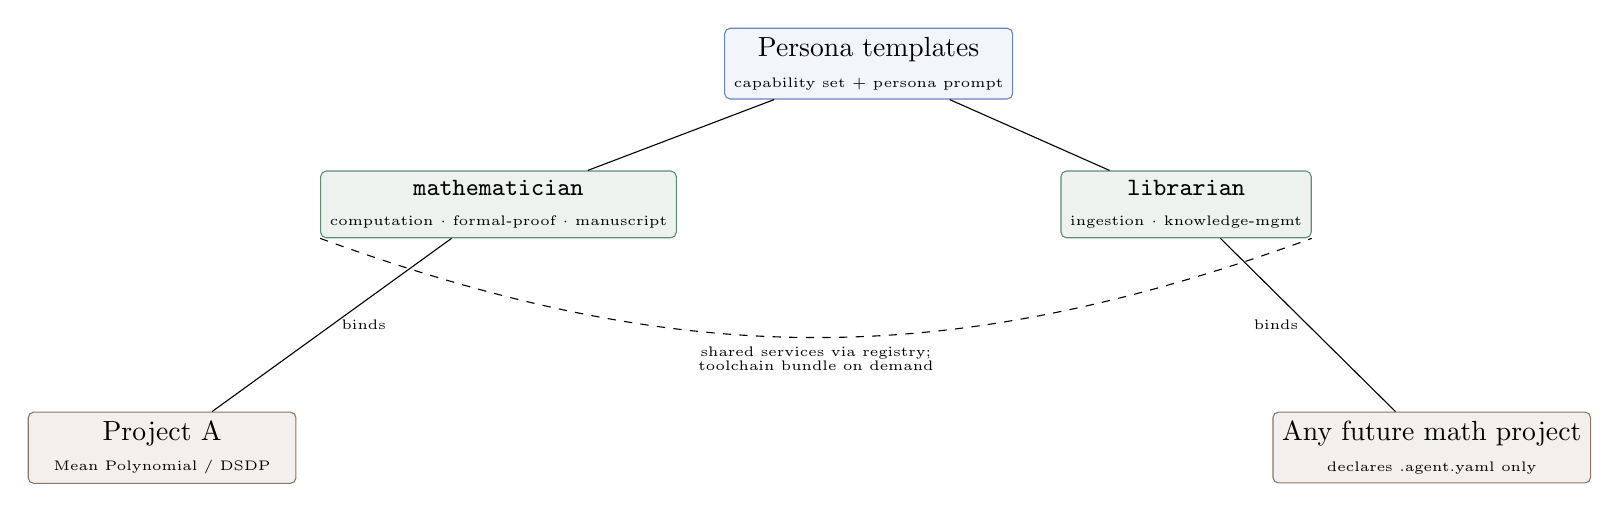
\begin{tikzpicture}[
    t/.style={draw=DarkBlue!60, fill=DarkBlue!5, rounded corners=2pt, minimum width=3.4cm, align=center},
    p/.style={draw=mathgreen!70, fill=mathgreen!8, rounded corners=2pt, minimum width=3.0cm, align=center},
    pr/.style={draw=libbrown!70, fill=libbrown!8, rounded corners=2pt, minimum width=3.4cm, align=center},
    every edge/.style={->, >=Stealth, draw=codegray}
  ]
  \node[t] (tmpl) {Persona templates\\[-1pt]\tiny capability set + persona prompt};
  \node[p, below left=0.9cm and 0.6cm of tmpl] (mathp) {\mono{mathematician}\\[-1pt]\tiny computation $\cdot$ formal-proof $\cdot$ manuscript};
  \node[p, below right=0.9cm and 0.6cm of tmpl] (libp) {\mono{librarian}\\[-1pt]\tiny ingestion $\cdot$ knowledge-mgmt};
  \node[pr, below left=2.2cm and 0.3cm of mathp] (projA) {Project A\\[-1pt]\tiny Mean Polynomial / DSDP};
  \node[pr, below right=2.2cm and -0.5cm of libp] (projB) {Any future math project\\[-1pt]\tiny declares .agent.yaml only};
  \draw (tmpl) -- (mathp); \draw (tmpl) -- (libp);
  \draw (mathp) -- node[right, font=\tiny]{binds} (projA);
  \draw (libp) -- node[left, font=\tiny]{binds} (projB);
  \draw [dashed] (mathp.south west) to[bend right=20] node[font=\tiny, align=center, below]{shared services via registry;\\[-1pt]toolchain bundle on demand} (libp.south east);
\end{tikzpicture}
\caption{Target model: personas are instantiated from templates with a capability set; projects bind
to personas through root-level binding files. No profile-internal configuration changes when the
project changes.}\label{fig:abstraction}
\end{figure}

%=====================================================================
\section{Roadmap for AgentDesign Itself}\label{sec:roadmap}

\begin{center}
\small
\renewcommand{\arraystretch}{1.2}
\begin{tabularx}{\textwidth}{@{}l X l@{}}
\toprule
Phase & Activity & Status\\
\midrule
I. Exploration & Read every config, skill tree, DB and script; extract data programmatically (\mono{references/extract\_profile\_data.py}) & done (2026-09-29)\\
II. Documentation & This document + \mono{skill\_inventory.md} + extracted JSON in \mono{data/} & this deliverable\\
III. Remediation PRs & The four one-line fixes of Section~\ref{sec:abstraction}(F), as separate commits against the live profiles & open\\
IV. Abstraction pilot & Implement capability frontmatter + loader gate for one skill pair (e.g.\ \mono{sagemath-mcp} under a test persona); verify librarian behavior is unchanged & open\\
V. Migration & Shared adapter move, services.yaml, toolchain bundle; then retire disabled lists & open\\
\bottomrule
\end{tabularx}
\end{center}

%=====================================================================
\section*{Sources and Verification}\label{sec:sources}

All facts in this document were read from the following locations on 2026-09-29 (config version
49); no claim was taken from memory:

\begin{itemize}
    \item \mono{\textasciitilde/.hermes/profiles/\{math,librarian\}/}: \mono{config.yaml}, \mono{.env}
    (values redacted in \mono{data/profile\_comparison.json}), \mono{profile.yaml}, \mono{state.db},
    \mono{cron/jobs.json}, \mono{scripts/}, \mono{plugins/}, \mono{home/}, full skill trees.
    \item \mono{\textasciitilde/.hermes/plugins/} (shared plugin installs),
    \mono{\textasciitilde/.hermes/mcp-servers/.venv/}.
    \item Extraction script and output: \mono{AgentDesign/references/extract\_profile\_data.py},
    \mono{AgentDesign/data/profile\_comparison.json}; skill inventory:
    \mono{AgentDesign/references/skill\_inventory.md}.
    \item Irene merge date (2026-09-18) and absence of \mono{hermes\_mcp\_tool.py} under the merged
    tree: filesystem check.
\end{itemize}

\textbf{Redaction note}: API keys, tokens and passwords appear in the source \mono{.env} files but
are masked as \mono{***} everywhere in this project's data artifacts; URLs, ports and paths are
recorded verbatim because they carry no secret value.

\end{document}
